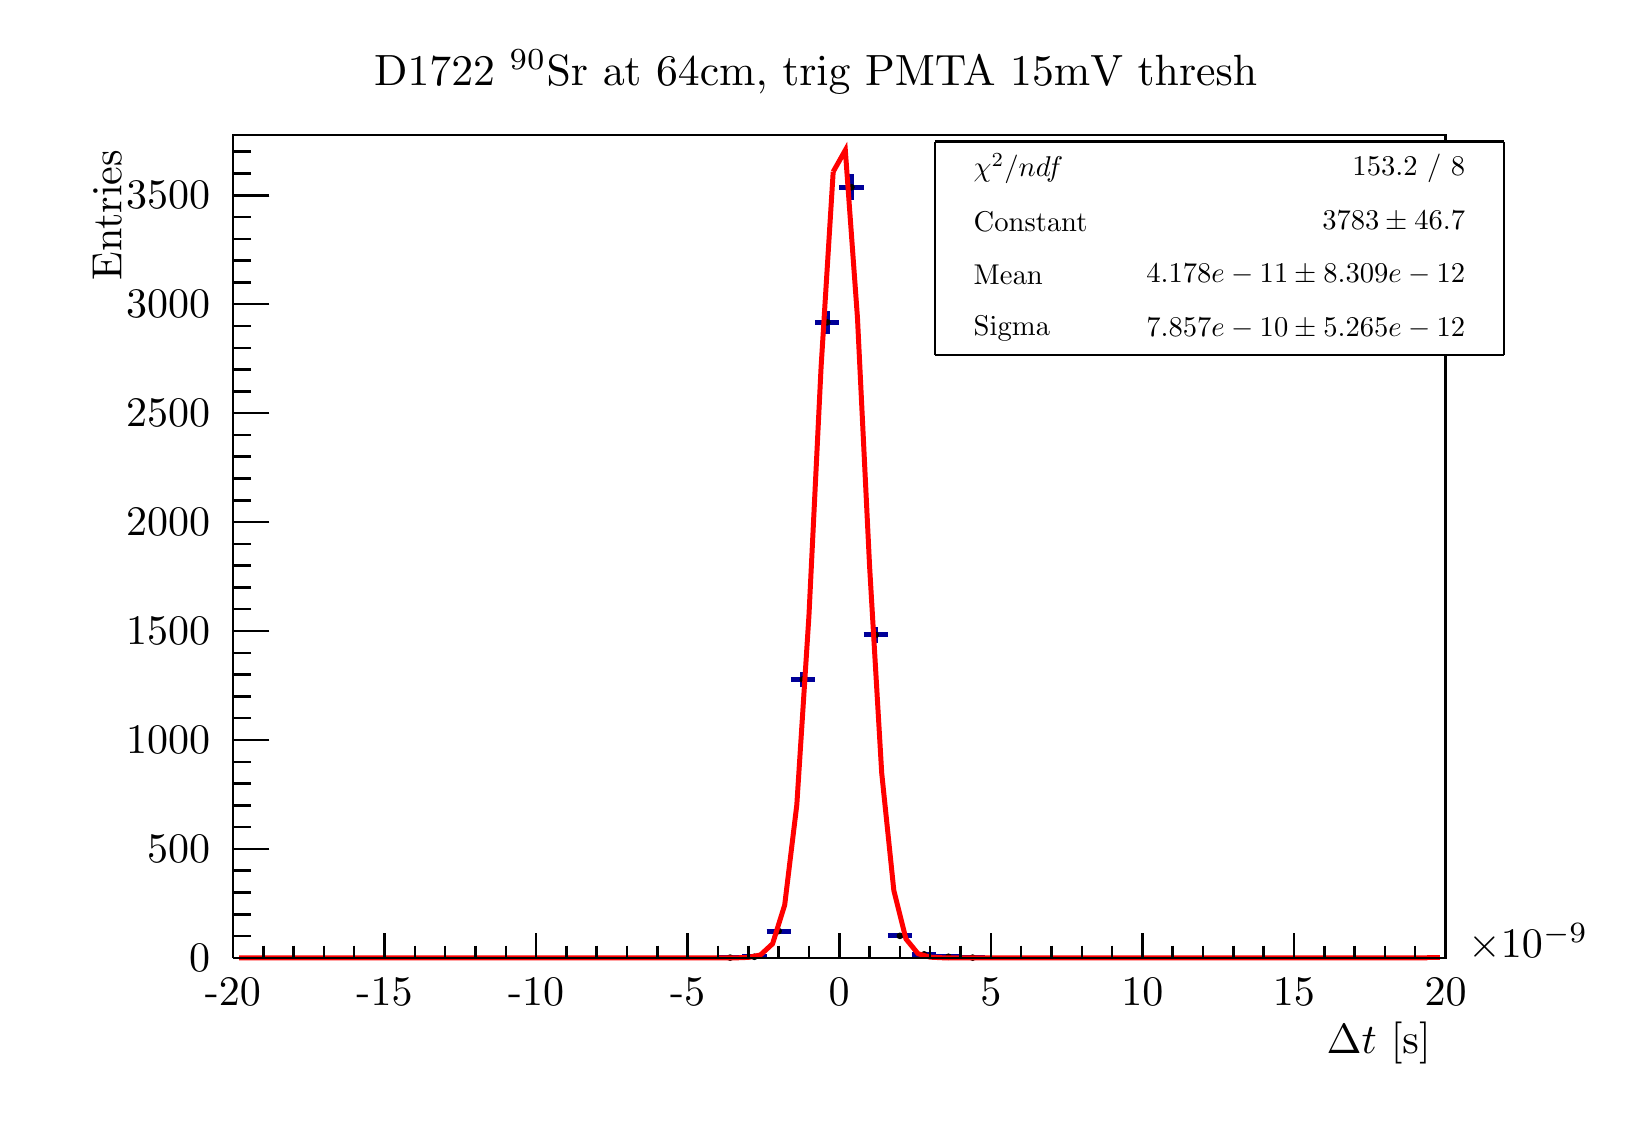
\begin{tikzpicture}
\pgfdeclareplotmark{cross} {
\pgfpathmoveto{\pgfpoint{-0.3\pgfplotmarksize}{\pgfplotmarksize}}
\pgfpathlineto{\pgfpoint{+0.3\pgfplotmarksize}{\pgfplotmarksize}}
\pgfpathlineto{\pgfpoint{+0.3\pgfplotmarksize}{0.3\pgfplotmarksize}}
\pgfpathlineto{\pgfpoint{+1\pgfplotmarksize}{0.3\pgfplotmarksize}}
\pgfpathlineto{\pgfpoint{+1\pgfplotmarksize}{-0.3\pgfplotmarksize}}
\pgfpathlineto{\pgfpoint{+0.3\pgfplotmarksize}{-0.3\pgfplotmarksize}}
\pgfpathlineto{\pgfpoint{+0.3\pgfplotmarksize}{-1.\pgfplotmarksize}}
\pgfpathlineto{\pgfpoint{-0.3\pgfplotmarksize}{-1.\pgfplotmarksize}}
\pgfpathlineto{\pgfpoint{-0.3\pgfplotmarksize}{-0.3\pgfplotmarksize}}
\pgfpathlineto{\pgfpoint{-1.\pgfplotmarksize}{-0.3\pgfplotmarksize}}
\pgfpathlineto{\pgfpoint{-1.\pgfplotmarksize}{0.3\pgfplotmarksize}}
\pgfpathlineto{\pgfpoint{-0.3\pgfplotmarksize}{0.3\pgfplotmarksize}}
\pgfpathclose
\pgfusepathqstroke
}
\pgfdeclareplotmark{cross*} {
\pgfpathmoveto{\pgfpoint{-0.3\pgfplotmarksize}{\pgfplotmarksize}}
\pgfpathlineto{\pgfpoint{+0.3\pgfplotmarksize}{\pgfplotmarksize}}
\pgfpathlineto{\pgfpoint{+0.3\pgfplotmarksize}{0.3\pgfplotmarksize}}
\pgfpathlineto{\pgfpoint{+1\pgfplotmarksize}{0.3\pgfplotmarksize}}
\pgfpathlineto{\pgfpoint{+1\pgfplotmarksize}{-0.3\pgfplotmarksize}}
\pgfpathlineto{\pgfpoint{+0.3\pgfplotmarksize}{-0.3\pgfplotmarksize}}
\pgfpathlineto{\pgfpoint{+0.3\pgfplotmarksize}{-1.\pgfplotmarksize}}
\pgfpathlineto{\pgfpoint{-0.3\pgfplotmarksize}{-1.\pgfplotmarksize}}
\pgfpathlineto{\pgfpoint{-0.3\pgfplotmarksize}{-0.3\pgfplotmarksize}}
\pgfpathlineto{\pgfpoint{-1.\pgfplotmarksize}{-0.3\pgfplotmarksize}}
\pgfpathlineto{\pgfpoint{-1.\pgfplotmarksize}{0.3\pgfplotmarksize}}
\pgfpathlineto{\pgfpoint{-0.3\pgfplotmarksize}{0.3\pgfplotmarksize}}
\pgfpathclose
\pgfusepathqfillstroke
}
\pgfdeclareplotmark{newstar} {
\pgfpathmoveto{\pgfqpoint{0pt}{\pgfplotmarksize}}
\pgfpathlineto{\pgfqpointpolar{44}{0.5\pgfplotmarksize}}
\pgfpathlineto{\pgfqpointpolar{18}{\pgfplotmarksize}}
\pgfpathlineto{\pgfqpointpolar{-20}{0.5\pgfplotmarksize}}
\pgfpathlineto{\pgfqpointpolar{-54}{\pgfplotmarksize}}
\pgfpathlineto{\pgfqpointpolar{-90}{0.5\pgfplotmarksize}}
\pgfpathlineto{\pgfqpointpolar{234}{\pgfplotmarksize}}
\pgfpathlineto{\pgfqpointpolar{198}{0.5\pgfplotmarksize}}
\pgfpathlineto{\pgfqpointpolar{162}{\pgfplotmarksize}}
\pgfpathlineto{\pgfqpointpolar{134}{0.5\pgfplotmarksize}}
\pgfpathclose
\pgfusepathqstroke
}
\pgfdeclareplotmark{newstar*} {
\pgfpathmoveto{\pgfqpoint{0pt}{\pgfplotmarksize}}
\pgfpathlineto{\pgfqpointpolar{44}{0.5\pgfplotmarksize}}
\pgfpathlineto{\pgfqpointpolar{18}{\pgfplotmarksize}}
\pgfpathlineto{\pgfqpointpolar{-20}{0.5\pgfplotmarksize}}
\pgfpathlineto{\pgfqpointpolar{-54}{\pgfplotmarksize}}
\pgfpathlineto{\pgfqpointpolar{-90}{0.5\pgfplotmarksize}}
\pgfpathlineto{\pgfqpointpolar{234}{\pgfplotmarksize}}
\pgfpathlineto{\pgfqpointpolar{198}{0.5\pgfplotmarksize}}
\pgfpathlineto{\pgfqpointpolar{162}{\pgfplotmarksize}}
\pgfpathlineto{\pgfqpointpolar{134}{0.5\pgfplotmarksize}}
\pgfpathclose
\pgfusepathqfillstroke
}
\definecolor{c}{rgb}{1,1,1};
\draw [color=c, fill=c] (0,0) rectangle (20,13.5705);
\draw [color=c, fill=c] (2.6,1.76416) rectangle (18,12.2134);
\definecolor{c}{rgb}{0,0,0};
\draw [c,line width=0.9] (2.6,1.76416) -- (2.6,12.2134) -- (18,12.2134) -- (18,1.76416) -- (2.6,1.76416);
\definecolor{c}{rgb}{1,1,1};
\draw [color=c, fill=c] (2.6,1.76416) rectangle (18,12.2134);
\definecolor{c}{rgb}{0,0,0};
\draw [c,line width=0.9] (2.6,1.76416) -- (2.6,12.2134) -- (18,12.2134) -- (18,1.76416) -- (2.6,1.76416);
\definecolor{c}{rgb}{0,0,0.6};
\draw [c,line width=1.8] (8.914,1.76416) -- (8.914,1.76693);
\draw [c,line width=1.8] (8.914,1.76693) -- (8.914,1.76969);
\draw [c,line width=1.8] (8.76,1.76693) -- (8.914,1.76693);
\draw [c,line width=1.8] (8.914,1.76693) -- (9.068,1.76693);
\definecolor{c}{rgb}{0,0,0};
\foreach \P in {(8.914,1.76693)}{\draw[mark options={color=c,fill=c},mark size=2.402402pt,mark=*,mark size=1pt] plot coordinates {\P};}
\definecolor{c}{rgb}{0,0,0.6};
\draw [c,line width=1.8] (9.222,1.77181) -- (9.222,1.77799);
\draw [c,line width=1.8] (9.222,1.77799) -- (9.222,1.78418);
\draw [c,line width=1.8] (9.068,1.77799) -- (9.222,1.77799);
\draw [c,line width=1.8] (9.222,1.77799) -- (9.376,1.77799);
\definecolor{c}{rgb}{0,0,0};
\foreach \P in {(9.222,1.77799)}{\draw[mark options={color=c,fill=c},mark size=2.402402pt,mark=*,mark size=1pt] plot coordinates {\P};}
\definecolor{c}{rgb}{0,0,0.6};
\draw [c,line width=1.8] (9.53,2.07382) -- (9.53,2.10451);
\draw [c,line width=1.8] (9.53,2.10451) -- (9.53,2.1352);
\draw [c,line width=1.8] (9.376,2.10451) -- (9.53,2.10451);
\draw [c,line width=1.8] (9.53,2.10451) -- (9.684,2.10451);
\definecolor{c}{rgb}{0,0,0};
\foreach \P in {(9.53,2.10451)}{\draw[mark options={color=c,fill=c},mark size=2.402402pt,mark=*,mark size=1pt] plot coordinates {\P};}
\definecolor{c}{rgb}{0,0,0.6};
\draw [c,line width=1.8] (9.838,5.20154) -- (9.838,5.30046);
\draw [c,line width=1.8] (9.838,5.30046) -- (9.838,5.39938);
\draw [c,line width=1.8] (9.684,5.30046) -- (9.838,5.30046);
\draw [c,line width=1.8] (9.838,5.30046) -- (9.992,5.30046);
\definecolor{c}{rgb}{0,0,0};
\foreach \P in {(9.838,5.30046)}{\draw[mark options={color=c,fill=c},mark size=2.402402pt,mark=*,mark size=1pt] plot coordinates {\P};}
\definecolor{c}{rgb}{0,0,0.6};
\draw [c,line width=1.8] (10.146,9.68623) -- (10.146,9.83568);
\draw [c,line width=1.8] (10.146,9.83568) -- (10.146,9.98513);
\draw [c,line width=1.8] (9.992,9.83568) -- (10.146,9.83568);
\draw [c,line width=1.8] (10.146,9.83568) -- (10.3,9.83568);
\definecolor{c}{rgb}{0,0,0};
\foreach \P in {(10.146,9.83568)}{\draw[mark options={color=c,fill=c},mark size=2.402402pt,mark=*,mark size=1pt] plot coordinates {\P};}
\definecolor{c}{rgb}{0,0,0.6};
\draw [c,line width=1.8] (10.454,11.3867) -- (10.454,11.5513);
\draw [c,line width=1.8] (10.454,11.5513) -- (10.454,11.7158);
\draw [c,line width=1.8] (10.3,11.5513) -- (10.454,11.5513);
\draw [c,line width=1.8] (10.454,11.5513) -- (10.608,11.5513);
\definecolor{c}{rgb}{0,0,0};
\foreach \P in {(10.454,11.5513)}{\draw[mark options={color=c,fill=c},mark size=2.402402pt,mark=*,mark size=1pt] plot coordinates {\P};}
\definecolor{c}{rgb}{0,0,0.6};
\draw [c,line width=1.8] (10.762,5.75842) -- (10.762,5.86495);
\draw [c,line width=1.8] (10.762,5.86495) -- (10.762,5.97147);
\draw [c,line width=1.8] (10.608,5.86495) -- (10.762,5.86495);
\draw [c,line width=1.8] (10.762,5.86495) -- (10.916,5.86495);
\definecolor{c}{rgb}{0,0,0};
\foreach \P in {(10.762,5.86495)}{\draw[mark options={color=c,fill=c},mark size=2.402402pt,mark=*,mark size=1pt] plot coordinates {\P};}
\definecolor{c}{rgb}{0,0,0.6};
\draw [c,line width=1.8] (11.07,2.01582) -- (11.07,2.04363);
\draw [c,line width=1.8] (11.07,2.04363) -- (11.07,2.07144);
\draw [c,line width=1.8] (10.916,2.04363) -- (11.07,2.04363);
\draw [c,line width=1.8] (11.07,2.04363) -- (11.224,2.04363);
\definecolor{c}{rgb}{0,0,0};
\foreach \P in {(11.07,2.04363)}{\draw[mark options={color=c,fill=c},mark size=2.402402pt,mark=*,mark size=1pt] plot coordinates {\P};}
\definecolor{c}{rgb}{0,0,0.6};
\draw [c,line width=1.8] (11.378,1.79736) -- (11.378,1.80843);
\draw [c,line width=1.8] (11.378,1.80843) -- (11.378,1.8195);
\draw [c,line width=1.8] (11.224,1.80843) -- (11.378,1.80843);
\draw [c,line width=1.8] (11.378,1.80843) -- (11.532,1.80843);
\definecolor{c}{rgb}{0,0,0};
\foreach \P in {(11.378,1.80843)}{\draw[mark options={color=c,fill=c},mark size=2.402402pt,mark=*,mark size=1pt] plot coordinates {\P};}
\definecolor{c}{rgb}{0,0,0.6};
\draw [c,line width=1.8] (11.686,1.77181) -- (11.686,1.77799);
\draw [c,line width=1.8] (11.686,1.77799) -- (11.686,1.78418);
\draw [c,line width=1.8] (11.532,1.77799) -- (11.686,1.77799);
\draw [c,line width=1.8] (11.686,1.77799) -- (11.84,1.77799);
\definecolor{c}{rgb}{0,0,0};
\foreach \P in {(11.686,1.77799)}{\draw[mark options={color=c,fill=c},mark size=2.402402pt,mark=*,mark size=1pt] plot coordinates {\P};}
\definecolor{c}{rgb}{0,0,0.6};
\draw [c,line width=1.8] (11.994,1.76416) -- (11.994,1.76693);
\draw [c,line width=1.8] (11.994,1.76693) -- (11.994,1.76969);
\draw [c,line width=1.8] (11.84,1.76693) -- (11.994,1.76693);
\draw [c,line width=1.8] (11.994,1.76693) -- (12.148,1.76693);
\definecolor{c}{rgb}{0,0,0};
\foreach \P in {(11.994,1.76693)}{\draw[mark options={color=c,fill=c},mark size=2.402402pt,mark=*,mark size=1pt] plot coordinates {\P};}
\definecolor{c}{rgb}{1,0,0};
\draw [c,line width=1.8] (2.677,1.76416) -- (2.831,1.76416) -- (2.985,1.76416) -- (3.139,1.76416) -- (3.293,1.76416) -- (3.447,1.76416) -- (3.601,1.76416) -- (3.755,1.76416) -- (3.909,1.76416) -- (4.063,1.76416) -- (4.217,1.76416) -- (4.371,1.76416)
 -- (4.525,1.76416) -- (4.679,1.76416) -- (4.833,1.76416) -- (4.987,1.76416) -- (5.141,1.76416) -- (5.295,1.76416) -- (5.449,1.76416) -- (5.603,1.76416) -- (5.757,1.76416) -- (5.911,1.76416) -- (6.065,1.76416) -- (6.219,1.76416) -- (6.373,1.76416) --
 (6.527,1.76416) -- (6.681,1.76416) -- (6.835,1.76416) -- (6.989,1.76416) -- (7.143,1.76416) -- (7.297,1.76416) -- (7.451,1.76416) -- (7.605,1.76416) -- (7.759,1.76416) -- (7.913,1.76416) -- (8.067,1.76416) -- (8.221,1.76416) -- (8.375,1.76416) --
 (8.529,1.76416) -- (8.683,1.76416) -- (8.837,1.76416) -- (8.991,1.76416) -- (9.145,1.76998) -- (9.299,1.80089) -- (9.453,1.94285) -- (9.607,2.43506) -- (9.761,3.70796) -- (9.915,6.11015) -- (10.069,9.26248) -- (10.223,11.7476);
\draw [c,line width=1.8] (10.223,11.7476) -- (10.377,12.0215) -- (10.531,9.89679) -- (10.685,6.74) -- (10.839,4.11347) -- (10.993,2.62012) -- (11.147,2.00482) -- (11.301,1.81637) -- (11.455,1.7729) -- (11.609,1.76529) -- (11.763,1.76416) --
 (11.917,1.76416) -- (12.071,1.76416) -- (12.225,1.76416) -- (12.379,1.76416) -- (12.533,1.76416) -- (12.687,1.76416) -- (12.841,1.76416) -- (12.995,1.76416) -- (13.149,1.76416) -- (13.303,1.76416) -- (13.457,1.76416) -- (13.611,1.76416) --
 (13.765,1.76416) -- (13.919,1.76416) -- (14.073,1.76416) -- (14.227,1.76416) -- (14.381,1.76416) -- (14.535,1.76416) -- (14.689,1.76416) -- (14.843,1.76416) -- (14.997,1.76416) -- (15.151,1.76416) -- (15.305,1.76416) -- (15.459,1.76416) --
 (15.613,1.76416) -- (15.767,1.76416) -- (15.921,1.76416) -- (16.075,1.76416) -- (16.229,1.76416) -- (16.383,1.76416) -- (16.537,1.76416) -- (16.691,1.76416) -- (16.845,1.76416) -- (16.999,1.76416) -- (17.153,1.76416) -- (17.307,1.76416) --
 (17.461,1.76416) -- (17.615,1.76416) -- (17.769,1.76416);
\draw [c,line width=1.8] (17.769,1.76416) -- (17.923,1.76416);
\definecolor{c}{rgb}{1,1,1};
\draw [color=c, fill=c] (11.5186,9.42152) rectangle (18.7393,12.1299);
\definecolor{c}{rgb}{0,0,0};
\draw [c,line width=0.9] (11.5186,9.42152) -- (18.7393,9.42152);
\draw [c,line width=0.9] (18.7393,9.42152) -- (18.7393,12.1299);
\draw [c,line width=0.9] (18.7393,12.1299) -- (11.5186,12.1299);
\draw [c,line width=0.9] (11.5186,12.1299) -- (11.5186,9.42152);
\draw [anchor= west] (11.8797,11.7913) node[scale=1.03301, color=c, rotate=0]{$\chi^{2} / ndf $};
\draw [anchor= east] (18.3782,11.7913) node[scale=1.03301, color=c, rotate=0]{ 153.2 / 8};
\draw [anchor= west] (11.8797,11.1142) node[scale=1.03301, color=c, rotate=0]{Constant };
\draw [anchor= east] (18.3782,11.1142) node[scale=1.03301, color=c, rotate=0]{$  3783 \pm 46.7$};
\draw [anchor= west] (11.8797,10.4371) node[scale=1.03301, color=c, rotate=0]{Mean     };
\draw [anchor= east] (18.3782,10.4371) node[scale=1.03301, color=c, rotate=0]{$ 4.178e-11 \pm 8.309e-12$};
\draw [anchor= west] (11.8797,9.76007) node[scale=1.03301, color=c, rotate=0]{Sigma    };
\draw [anchor= east] (18.3782,9.76007) node[scale=1.03301, color=c, rotate=0]{$ 7.857e-10 \pm 5.265e-12$};
\draw [c,line width=0.9] (2.6,1.76416) -- (18,1.76416);
\draw [c,line width=0.9] (2.6,2.07764) -- (2.6,1.76416);
\draw [c,line width=0.9] (2.985,1.9209) -- (2.985,1.76416);
\draw [c,line width=0.9] (3.37,1.9209) -- (3.37,1.76416);
\draw [c,line width=0.9] (3.755,1.9209) -- (3.755,1.76416);
\draw [c,line width=0.9] (4.14,1.9209) -- (4.14,1.76416);
\draw [c,line width=0.9] (4.525,2.07764) -- (4.525,1.76416);
\draw [c,line width=0.9] (4.91,1.9209) -- (4.91,1.76416);
\draw [c,line width=0.9] (5.295,1.9209) -- (5.295,1.76416);
\draw [c,line width=0.9] (5.68,1.9209) -- (5.68,1.76416);
\draw [c,line width=0.9] (6.065,1.9209) -- (6.065,1.76416);
\draw [c,line width=0.9] (6.45,2.07764) -- (6.45,1.76416);
\draw [c,line width=0.9] (6.835,1.9209) -- (6.835,1.76416);
\draw [c,line width=0.9] (7.22,1.9209) -- (7.22,1.76416);
\draw [c,line width=0.9] (7.605,1.9209) -- (7.605,1.76416);
\draw [c,line width=0.9] (7.99,1.9209) -- (7.99,1.76416);
\draw [c,line width=0.9] (8.375,2.07764) -- (8.375,1.76416);
\draw [c,line width=0.9] (8.76,1.9209) -- (8.76,1.76416);
\draw [c,line width=0.9] (9.145,1.9209) -- (9.145,1.76416);
\draw [c,line width=0.9] (9.53,1.9209) -- (9.53,1.76416);
\draw [c,line width=0.9] (9.915,1.9209) -- (9.915,1.76416);
\draw [c,line width=0.9] (10.3,2.07764) -- (10.3,1.76416);
\draw [c,line width=0.9] (10.685,1.9209) -- (10.685,1.76416);
\draw [c,line width=0.9] (11.07,1.9209) -- (11.07,1.76416);
\draw [c,line width=0.9] (11.455,1.9209) -- (11.455,1.76416);
\draw [c,line width=0.9] (11.84,1.9209) -- (11.84,1.76416);
\draw [c,line width=0.9] (12.225,2.07764) -- (12.225,1.76416);
\draw [c,line width=0.9] (12.61,1.9209) -- (12.61,1.76416);
\draw [c,line width=0.9] (12.995,1.9209) -- (12.995,1.76416);
\draw [c,line width=0.9] (13.38,1.9209) -- (13.38,1.76416);
\draw [c,line width=0.9] (13.765,1.9209) -- (13.765,1.76416);
\draw [c,line width=0.9] (14.15,2.07764) -- (14.15,1.76416);
\draw [c,line width=0.9] (14.535,1.9209) -- (14.535,1.76416);
\draw [c,line width=0.9] (14.92,1.9209) -- (14.92,1.76416);
\draw [c,line width=0.9] (15.305,1.9209) -- (15.305,1.76416);
\draw [c,line width=0.9] (15.69,1.9209) -- (15.69,1.76416);
\draw [c,line width=0.9] (16.075,2.07764) -- (16.075,1.76416);
\draw [c,line width=0.9] (16.46,1.9209) -- (16.46,1.76416);
\draw [c,line width=0.9] (16.845,1.9209) -- (16.845,1.76416);
\draw [c,line width=0.9] (17.23,1.9209) -- (17.23,1.76416);
\draw [c,line width=0.9] (17.615,1.9209) -- (17.615,1.76416);
\draw [c,line width=0.9] (18,2.07764) -- (18,1.76416);
\draw [anchor=base] (2.6,1.15349) node[scale=1.51913, color=c, rotate=0]{-20};
\draw [anchor=base] (4.525,1.15349) node[scale=1.51913, color=c, rotate=0]{-15};
\draw [anchor=base] (6.45,1.15349) node[scale=1.51913, color=c, rotate=0]{-10};
\draw [anchor=base] (8.375,1.15349) node[scale=1.51913, color=c, rotate=0]{-5};
\draw [anchor=base] (10.3,1.15349) node[scale=1.51913, color=c, rotate=0]{0};
\draw [anchor=base] (12.225,1.15349) node[scale=1.51913, color=c, rotate=0]{5};
\draw [anchor=base] (14.15,1.15349) node[scale=1.51913, color=c, rotate=0]{10};
\draw [anchor=base] (16.075,1.15349) node[scale=1.51913, color=c, rotate=0]{15};
\draw [anchor=base] (18,1.15349) node[scale=1.51913, color=c, rotate=0]{20};
\draw [anchor=base west] (18.1,1.76416) node[scale=1.51913, color=c, rotate=0]{$\times10^{-9}$};
\draw [anchor= east] (18,0.678523) node[scale=1.51913, color=c, rotate=0]{$\Delta t$ [s]};
\draw [c,line width=0.9] (2.6,1.76416) -- (2.6,12.2134);
\draw [c,line width=0.9] (3.062,1.76416) -- (2.6,1.76416);
\draw [c,line width=0.9] (2.831,2.04086) -- (2.6,2.04086);
\draw [c,line width=0.9] (2.831,2.31757) -- (2.6,2.31757);
\draw [c,line width=0.9] (2.831,2.59428) -- (2.6,2.59428);
\draw [c,line width=0.9] (2.831,2.87098) -- (2.6,2.87098);
\draw [c,line width=0.9] (3.062,3.14769) -- (2.6,3.14769);
\draw [c,line width=0.9] (2.831,3.4244) -- (2.6,3.4244);
\draw [c,line width=0.9] (2.831,3.7011) -- (2.6,3.7011);
\draw [c,line width=0.9] (2.831,3.97781) -- (2.6,3.97781);
\draw [c,line width=0.9] (2.831,4.25451) -- (2.6,4.25451);
\draw [c,line width=0.9] (3.062,4.53122) -- (2.6,4.53122);
\draw [c,line width=0.9] (2.831,4.80793) -- (2.6,4.80793);
\draw [c,line width=0.9] (2.831,5.08463) -- (2.6,5.08463);
\draw [c,line width=0.9] (2.831,5.36134) -- (2.6,5.36134);
\draw [c,line width=0.9] (2.831,5.63805) -- (2.6,5.63805);
\draw [c,line width=0.9] (3.062,5.91475) -- (2.6,5.91475);
\draw [c,line width=0.9] (2.831,6.19146) -- (2.6,6.19146);
\draw [c,line width=0.9] (2.831,6.46816) -- (2.6,6.46816);
\draw [c,line width=0.9] (2.831,6.74487) -- (2.6,6.74487);
\draw [c,line width=0.9] (2.831,7.02158) -- (2.6,7.02158);
\draw [c,line width=0.9] (3.062,7.29828) -- (2.6,7.29828);
\draw [c,line width=0.9] (2.831,7.57499) -- (2.6,7.57499);
\draw [c,line width=0.9] (2.831,7.8517) -- (2.6,7.8517);
\draw [c,line width=0.9] (2.831,8.1284) -- (2.6,8.1284);
\draw [c,line width=0.9] (2.831,8.40511) -- (2.6,8.40511);
\draw [c,line width=0.9] (3.062,8.68182) -- (2.6,8.68182);
\draw [c,line width=0.9] (2.831,8.95852) -- (2.6,8.95852);
\draw [c,line width=0.9] (2.831,9.23523) -- (2.6,9.23523);
\draw [c,line width=0.9] (2.831,9.51193) -- (2.6,9.51193);
\draw [c,line width=0.9] (2.831,9.78864) -- (2.6,9.78864);
\draw [c,line width=0.9] (3.062,10.0653) -- (2.6,10.0653);
\draw [c,line width=0.9] (2.831,10.3421) -- (2.6,10.3421);
\draw [c,line width=0.9] (2.831,10.6188) -- (2.6,10.6188);
\draw [c,line width=0.9] (2.831,10.8955) -- (2.6,10.8955);
\draw [c,line width=0.9] (2.831,11.1722) -- (2.6,11.1722);
\draw [c,line width=0.9] (3.062,11.4489) -- (2.6,11.4489);
\draw [c,line width=0.9] (3.062,11.4489) -- (2.6,11.4489);
\draw [c,line width=0.9] (2.831,11.7256) -- (2.6,11.7256);
\draw [c,line width=0.9] (2.831,12.0023) -- (2.6,12.0023);
\draw [anchor= east] (2.5,1.76416) node[scale=1.51913, color=c, rotate=0]{0};
\draw [anchor= east] (2.5,3.14769) node[scale=1.51913, color=c, rotate=0]{500};
\draw [anchor= east] (2.5,4.53122) node[scale=1.51913, color=c, rotate=0]{1000};
\draw [anchor= east] (2.5,5.91475) node[scale=1.51913, color=c, rotate=0]{1500};
\draw [anchor= east] (2.5,7.29828) node[scale=1.51913, color=c, rotate=0]{2000};
\draw [anchor= east] (2.5,8.68182) node[scale=1.51913, color=c, rotate=0]{2500};
\draw [anchor= east] (2.5,10.0653) node[scale=1.51913, color=c, rotate=0]{3000};
\draw [anchor= east] (2.5,11.4489) node[scale=1.51913, color=c, rotate=0]{3500};
\draw [anchor= east] (1,12.2134) node[scale=1.51913, color=c, rotate=90]{Entries};
\definecolor{c}{rgb}{1,1,1};
\draw [color=c, fill=c] (11.5186,9.42152) rectangle (18.7393,12.1299);
\definecolor{c}{rgb}{0,0,0};
\draw [c,line width=0.9] (11.5186,9.42152) -- (18.7393,9.42152);
\draw [c,line width=0.9] (18.7393,9.42152) -- (18.7393,12.1299);
\draw [c,line width=0.9] (18.7393,12.1299) -- (11.5186,12.1299);
\draw [c,line width=0.9] (11.5186,12.1299) -- (11.5186,9.42152);
\draw [anchor= west] (11.8797,11.7913) node[scale=1.03301, color=c, rotate=0]{$\chi^{2} / ndf $};
\draw [anchor= east] (18.3782,11.7913) node[scale=1.03301, color=c, rotate=0]{ 153.2 / 8};
\draw [anchor= west] (11.8797,11.1142) node[scale=1.03301, color=c, rotate=0]{Constant };
\draw [anchor= east] (18.3782,11.1142) node[scale=1.03301, color=c, rotate=0]{$  3783 \pm 46.7$};
\draw [anchor= west] (11.8797,10.4371) node[scale=1.03301, color=c, rotate=0]{Mean     };
\draw [anchor= east] (18.3782,10.4371) node[scale=1.03301, color=c, rotate=0]{$ 4.178e-11 \pm 8.309e-12$};
\draw [anchor= west] (11.8797,9.76007) node[scale=1.03301, color=c, rotate=0]{Sigma    };
\draw [anchor= east] (18.3782,9.76007) node[scale=1.03301, color=c, rotate=0]{$ 7.857e-10 \pm 5.265e-12$};
\draw (10,13.0186) node[scale=1.5799, color=c, rotate=0]{D1722 $^{90}$Sr at 64cm, trig PMTA 15mV thresh};
\end{tikzpicture}
